\documentclass[a4paper,10pt]{article}

\usepackage{microtype}
\usepackage{pdfpages}
\usepackage{amsmath}
\usepackage{natbib}
\usepackage[margin=2.5cm]{geometry}
\usepackage{setspace}
  \doublespacing
\usepackage{enumitem}
  \setlist{nolistsep}
\usepackage{booktabs}
\usepackage{dcolumn}
  \newcolumntype{d}{D{.}{.}{5.1}}
\usepackage[utopia]{mathdesign}


\title{Proposed Design for a Cost-Effective and Energy-Efficient Wastewater Treatment System}
       
\author{Mohanadas Harish Chandar U067314J \\
       \normalsize{ESE3401 Water \& Wastewater Engineering 1 Mini-Project}}

\begin{document}
\maketitle


\section{Introduction}
A cost-effective and energy-efficient wastewater treatment system is proposed for a proposed estate by developer HOPE. 
The proposed treatment system is expected to provide tertiary level treatment for all wastewater generated from the estate's residential, institutional, commercial, and industrial developments. 
Effluent from the plant is expected to comply with Singapore's Trade Effluent Regulation (1976) standards for \emph{discharge into controlled watercourses}. 


\section{Background}
The client, HOPE, intends to develop an estate on a newly acquired piece of land. 
The proposed types and sizes of developments are given in Table~\ref{tab:developments-sizes}.

\begin{table}[htbp]
\centering
\begin{tabular}{l@{\qquad}d} \toprule
Type of development & \multicolumn{1}{c}{Land area allocated (ha)} \\ \midrule
Single family dwellings & 350 \\
Low-rise apartments & 450 \\
High-rise apartments & 900 \\
Commercial & 3200 \\
Industrial & 400 \\
School & 150 \\ \midrule
Total & 5450 \\ \bottomrule
\end{tabular}
\caption{Proposed types of development and land area allocated in estate.}
\label{tab:developments-sizes}
\end{table}

The Environmental Regulatory Agency's requirements are as follows:
\begin{itemize}
\item All wastewater generated is to be treated to meet the Singapore Trade Effluent Standards (1976)
\item All new treatment system are to cater to climate changes
\end{itemize}



\section{Key considerations}

\subsection{Design assumptions}
\subsubsection{Nature of sewer system}
The estate's sewer system is assumed to have separate and independently operating public sewers and storm drains. 
All wastewater from the public sewer will be treated by the proposed treatment system. 
Stormwater is assumed to be carried away by the storm drains into a nearby receiving body of adequate assimilation capacity.

\subsubsection{Industrial wastewater disposal}
\label{sec:industrial_wastewater_disposal}
Industries are assumed to have treated their wastewaste to meet Singapore's Trade Effluent Regulation (1976) standards for \emph{discharge into public sewers}.


\subsection{Operational considerations}
\subsubsection{Flowrate and loading estimates at carrying capacity}
Table~\ref{tab:population_flowrate} shows the estimated population and flowrate values at the estate's carrying capacity. Data is assumed to be based on similar nearby developments.

\begin{table}[htbp]
\begin{minipage}{\textwidth}
\renewcommand{\footnoterule}{}
\centering
\begin{tabular}{ldddddd} \toprule

Land use & \multicolumn{1}{c}{Land area} & \multicolumn{1}{c}{Population} & \multicolumn{1}{c}{Population} & \multicolumn{1}{c}{Per capita} & \multicolumn{1}{c}{Area} & \multicolumn{1}{c}{Design average} \\ 
 & \multicolumn{1}{c}{allocated} & \multicolumn{1}{c}{density$^a$} & \multicolumn{1}{c}{} & \multicolumn{1}{c}{flowrate$^b$} & \multicolumn{1}{c}{flowrate$^b$} & \multicolumn{1}{c}{flowrate} \\ 
 & \multicolumn{1}{c}{ (ha)} & \multicolumn{1}{c}{(capita/ha)} & \multicolumn{1}{c}{} & \multicolumn{1}{c}{(L/capita/d)} & \multicolumn{1}{c}{(m$^3$/ha/d)} & \multicolumn{1}{c}{(m$^3$/d)} \\ \midrule

Single-family & 350 & 50 & 17500 & 320 & 16 & 5600 \\ 
Low-rise & 450 & 150 & 67500 & 260 & 39 & 17550 \\ 
High-rise & 900 & 300 & 270000 & 200 & 60 & 54000 \\ \cmidrule{1-7}
Residential total & 1700 &  & 355000 &  &  & 77150 \\ 
 &  &  &  &  &  &  \\ 
Commercial & 3200 & 150 & 480000 & 50 & 7.5 & 24000 \\ 
Industrial & 400 & 100 & 40000 & 150 & 15 & 6000 \\ 
School & 150 & 400 & 60000 & 100 & 40 & 6000 \\ \cmidrule{1-7}
Other total & 3750 &  & 580000 &  &  & 36000 \\
 &  &  &  &  &  &  \\ 
Grand Total & 5450 &  &  &  &  & 113150 \\ \bottomrule
\end{tabular}
\footnotetext[1]{Population density is assumed to be estimated from similar nearby developments. Here it is deduced with information from \citep{Metropolitan2005}.}
\footnotetext[2]{Per capita and area flowrates are assumed to be estimated from similar nearby developments. Here they are based on typical values found in \citep{Metcalf2003}.}
\end{minipage}
\caption{Estimation of design average flowrate.}
\label{tab:population_flowrate}
\end{table}

\enlargethispage{\baselineskip}
\subsubsection{Startup and initial transition period}
\label{sec:startup_and_initial_transition_period}
In the initial months of treatment system operations, influent flowrates are expected to be to be well below design flowrates and rise steadily over time. 
Loading during this period is expected to undergo significant variablility due to major construction activities. 
The treatment system has to cater for this variability.

\subsubsection{Odour management}
Wastewater when gathered in large quantities is inherently odorous. Moreover, treatment processes themselves may produce odourous substances. The design should incorporate odour reduction technologies. 


\subsection{Cost effectiveness and energy efficiency}
\subsubsection{Modular design and progressive construction}
Flowrates during the initial transition period are expectied to be well below design flowrates. 
Thus, the full capacity of the treatment system does not need to be realised at the start of operations.
This allows the treatment system to be construction in a progressive manner. 

Cost-effectivesness is improved as the construction period can be lengthened, and the plant can operate close to optimum levels even in the initial transition period. 
To facilitate this, the treatment system will be designed in a modular fashion.

\subsubsection{Minimising land area requirements}
Treatment technologies that are compact and have small land requirements will be favoured.

\subsubsection{Reducing aeration requirements}
Experience has shown that aeration systems typically account for about 40--60\% of electricity usage in wastewater treatment systems. To improve energy efficiency, the treatment system will be designed to significantly reduce aeration requirements.

\subsubsection{Energy production from sludge handling}
\label{sec:energy_production_from_sludge_handling}
The scale of the treatment system allows anaerobic digestion to be performed in a cost-effective manner. The design will utilise biogas output from anaerobic sludge digestion to fulfil part of the treatment system's energy requirements.



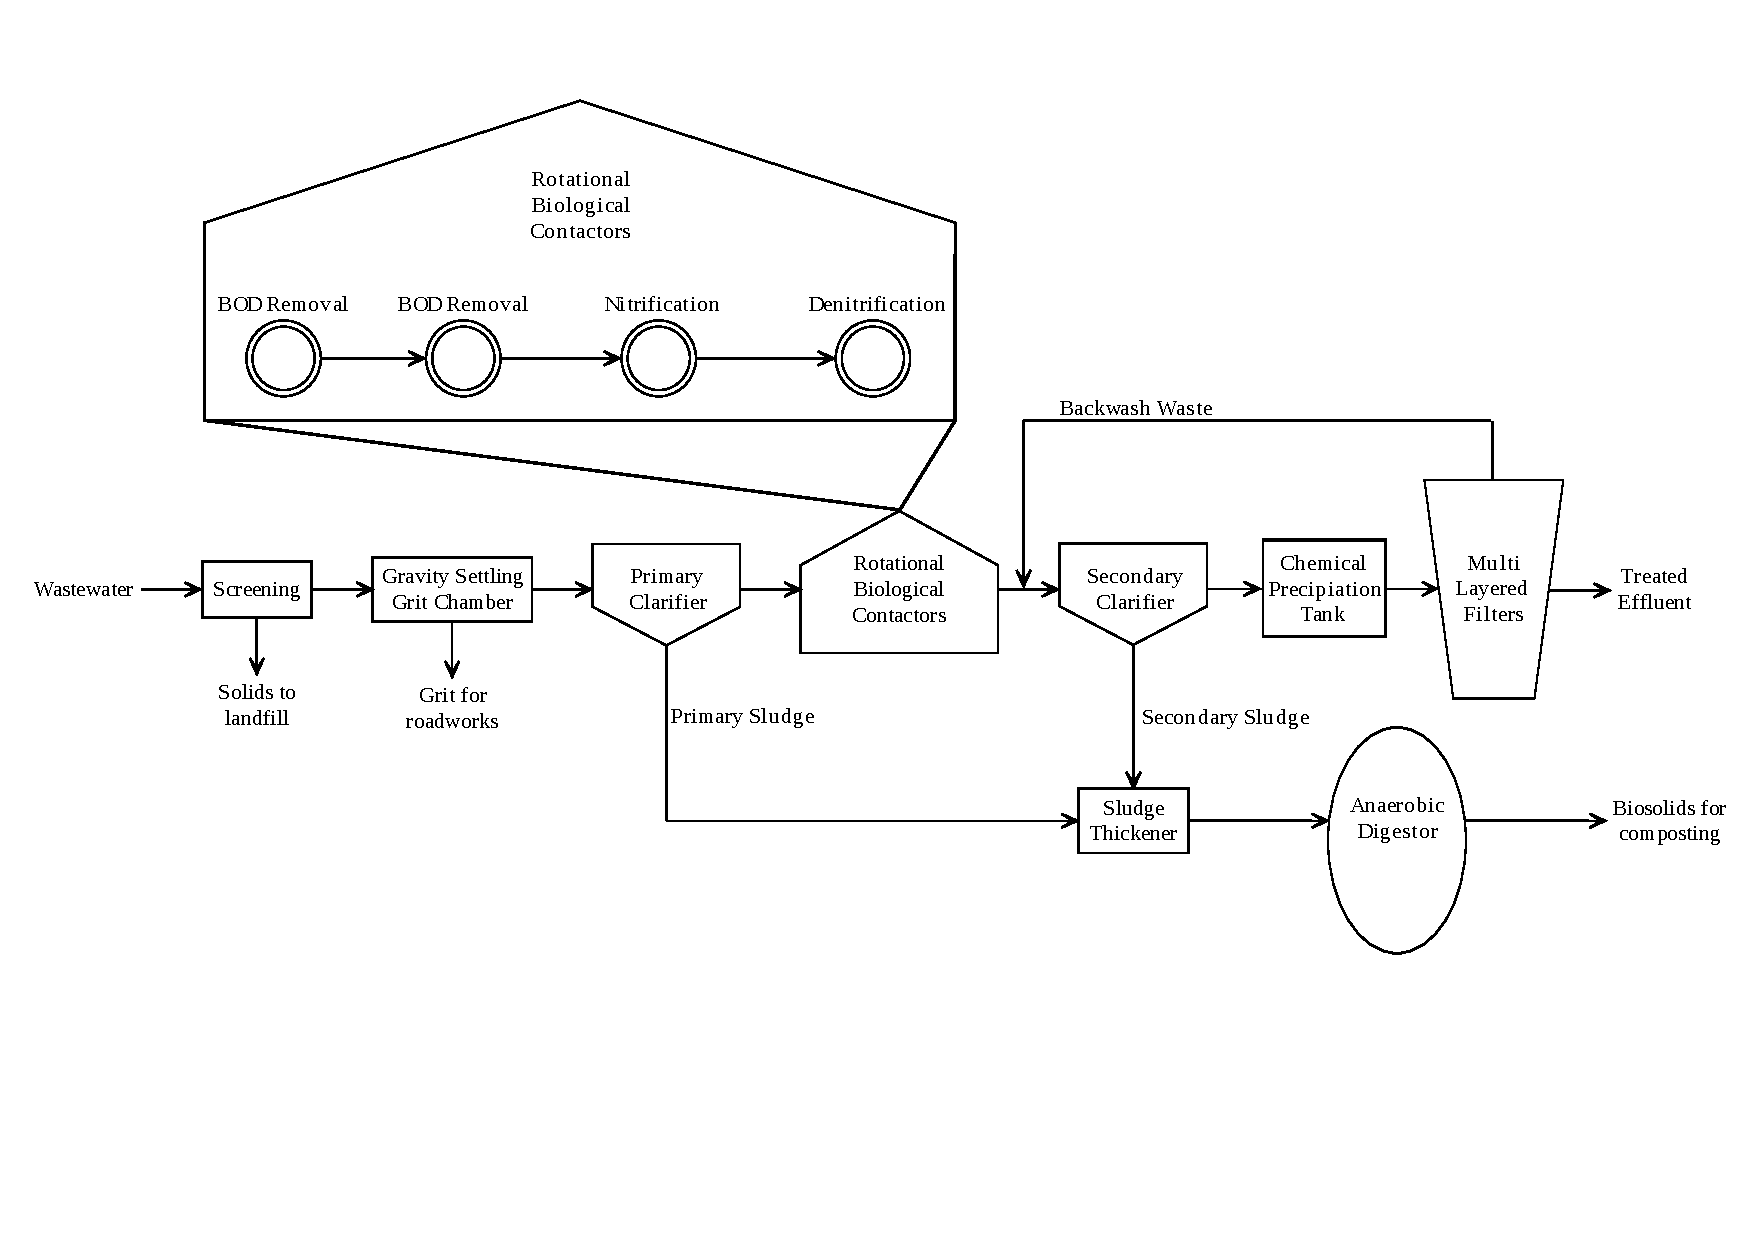
\includepdf[landscape]{diagram}


\section{Rationale for the proposed treatment system}
\subsection{Pre-treatment}
Large solids can damage treatment equipment.
Grit can abrade surfaces of treatment equipment, accumulate in pipes and tanks, and interfere with subsequent treatment processes. 
Grease forms a layer on the wastewater surface and prevents dissolving of atmospheric oxygen into the wastewater stream.
Pre-treatment removes large solids, grit and floatables such as grease from the influent stream.

\subsubsection{Mechanical bar screens}
Screening removes large solids and floatables such as branches, twigs, rags and cigarette butts, etc. Mechanical bar screens were chosen as they are cost-effective for a treatment system of this size.

Other options considered:
\begin{itemize}
\item Hand-cleaned bar screens
\end{itemize}

\subsubsection{Aerated grit chambers}
Aerated grit chambers were chosen for the following reasons:
\begin{itemize}
\item They are compact and occupy less space
\item Aeration removes odours, and facilitated subsequent BOD removal
\item The air bubbles dislodge organics from grit particles, allowing direct disposal of grit in landfills
\item Skimmers can be employed for grease removal
\item Greater control over particle settling can be achieved
\end{itemize}

Other options considered:
\begin{itemize}
\item Gravity settling grit chambers
\end{itemize}


\subsection{Primary treatment}
Primary treatment removes a portion of the SS and the BOD from the wastewater stream. This reduces loading on subsequent secondary treatment systems.

After primary treatment, 99\% of grit, 70\% of suspended solids (SS) and 20--40\% of BOD is expected to have been removed.

\subsubsection{Primary clarifiers}
\label{sec:primary_clarifiers}
Primary clarifiers were chosen as they are provide sufficient removal of SS and BOD while being cost-effective and energy-efficient. Detention time can be varied based on variations in loading and flowrates. Chemical additives can also be added if necessary.

Other options considered:
\begin{itemize}
\item Floatation systems
\end{itemize}


\subsection{Secondary treatment}
Secondary treatment removes most of the SS and BOD from the wastewater stream. Nitrogen removal is also included in this design. After secondary treatment, effluent SS and BOD concentration is expected to be about 15--30\,mg/L.

\subsubsection{Rotating biological contactors}
Rotating biological contactors (RBCs) were chosen as they are compact, and proven technology. RBC units can be arranged in series to promote specialization of bacteria, enhancing both BOD and nitrogen removal. RBCs are also cost-effectiveness and energy-efficiency as they usually do not require aeration. The modular nature of RBCs allows for more units to be added if required.

Other options considered:
\begin{itemize}
\item Activated-sludge process
\item Trickling filters
\item Stabilization lagoons
\item Anaerobic contact process
\end{itemize}

\subsubsection{Secondary clarifiers}
Secondary clarifiers remove waste sludge from the effluent stream after biological treatment. 
Secondary clarifies were chosen for the same reasons as primary clarifiers (see section~\ref{sec:primary_clarifiers}).

Other options considered:
\begin{itemize}
\item Floatation systems
\end{itemize}


\subsection{Tertiary treatment}
Tertiary treatment removes phosphorous and other trace constituents. Effluent is expected to meet Singapore's Trade Effluent Standards (1976) for \emph{discharge into controlled watercourses} after tertiary treatment.

\subsubsection{Chemical precipitation tanks}
The chemical precipitation tanks facilitate mixing of chemicals such as coagulants and neutralizing agents with the influent stream. This facilitates the subsequent filtration process.

\subsubsection{Multi layered filters}
When used with upstream coagulation, filtration can remove almost all remaining SS, nitrogen and phosphorus. Multi layered filters are chosen as they can function for a longer time than sand filters before backwash is necessary, and are more cost effective than filters with only activated carbon.

\begin{itemize}
\item Sand filters
\item Activated carbon filters
\end{itemize}


\subsection{Sludge handling}
\subsubsection{Sludge thinckeners}
Sludge thickeners remove water from the sludge stream. This reduces hydraulic loading on the digesters, making them more efficient in energy production per kg sludge processed.

\subsubsection{Anaerobic digestors}
Anaerobic digestion was chosen as it is both energy efficient and cost-effective for a treatment plant of this size. Removal of 40--60\% of organic solids is expected, reducing solid waste output. The biogas produced from the anaerobic digestion process can be used to fulfil part of the treatment system's energy requirements.

\bibliographystyle{apalike}
\bibliography{references}

\end{document}
